\chapter[Estado del arte y tecnologías utilizadas]{Estado del arte y tecnologías utilizadas}
\chaptermark{Arte y tecnologías}
\label{chap:estado del arte}

\section[Estado del arte de herramientas para monitorizar información]{Estado del arte de herramientas para monitorizar información}
\sectionmark{Estado del arte}





%\newpage
\section{Tecnologías utilizadas}

A continuación se detallan las diferentes tecnologías/bibliotecas/lenguajes que se han empleado para la elaboración del proyecto y por qué se han escogido por encima de otras posibles soluciones.


\subsection{\LaTeX}

Web: \url{https://www.latex-project.org/}\\

\LaTeX es un lenguaje de marcado que sirve para la redacción de documentos científicos o técnicos. Con esta herramienta o lenguaje se ha desarrollado la memoria actual del proyecto de final de carrera.



\subsection{PyCharm}

\hspace*{2.25in}{
\includegraphics[scale=0.25]{imagenes/pycharm-logo.png}}

Web: \url{https://www.jetbrains.com/pycharm/}\\

PyCharm es un IDE que permite el trabajo con aplicaciones Python en sus respectivos entornos virtuales (virtualenv) así como la integración con frameworks de desarrollo como es el caso de Django. La aplicación en sí fue desarrollada nativamente mediante un editor de texto (Emacs) pero a la hora de realizar un empaquetado e integración con otra herramientas se optó por este IDE. \\

\subsection{Bitbucket}

\hspace*{2in}{
\includegraphics{imagenes/bitbucket-logo.png}}\\

Web: \url{https://bitbucket.org/}\\
Repositorio: \url{https://bitbucket.org/MGautierGomez/securityproject}\\

Gestor de repositorios Git y Mercurial. Se optó por este gestor para probar su funcionamiento, así como la posibilidad de tener repositorios privados para desarrollar partes del proyecto que necesitasen ser ocultadas. También se encuentra alojado en el repositorio de \textbf{GitHub}: \url{https://github.com/MGautier/security-sensor}\\


\subsection{Git}

\hspace*{2.1in}{
\includegraphics[scale=0.5]{imagenes/git-logo.png}}

Web: \url{https://git-scm.com/}\\

Git es un sistema open-source de control de versiones diseñado para manejar integramente las fases de desarrollo de proyectos, simples y complejos, con velocidad y eficiencia.\\

\subsection{Digital Ocean}

\begin{center}
\includegraphics[scale=0.35]{imagenes/docean-logo.png}\end{center}

Web: \url{https://www.digitalocean.com/}\\

Servidor web para alojar proyectos en cloud. La ventaja de este servicio de VPS es que te permite desplegar máquinas de cualquier tipo (siempre que sean software libre) de una manera muy fácil y rápida. Además tiene un punto fuerte y es que la información se almacena en discos SSD, con lo que el procesamiento se ve muy mejorado a la hora de computar (en este caso eventos de Iptables).\\

\begin{figure}[H]
\hspace*{-1.5in}{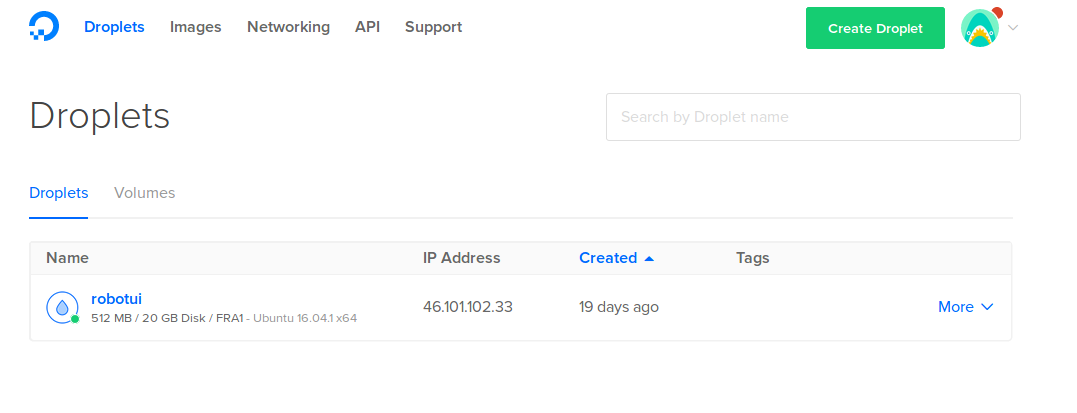
\includegraphics[scale=0.45]{imagenes/droplets.png}}
\caption{Droplet desplegado en digital ocean}
\end{figure}


